\section{Introduction:}

Zero crossing detectors are used to detect the types of signals, or different meanings of signals. Something very simple would be to consider a signal that 'in its positive part' will indicate a 'logical one' and in its negative part a 'logical zero'. The zero crossing detector is part of the detection circuit 'by level' to determine if a 'one' or a 'zero' has been received. With analog signals the zero crossing detectors operate with waveform much more variants than those of the digital case, they can be used to determine the type of the waveform, the average level of the signal, help integrate or differentiate signals, etc. All that 'mathematical function' to apply to the signal that requires determining the 'zero level' of such a signal. A practical example of this configuration is the zero-crossing inverting and non-inverting detectors showed in Figures 1.0 and 1.2 respectively. \hfill \break

\begin{multicols}{2}
\begin{figure}[H]
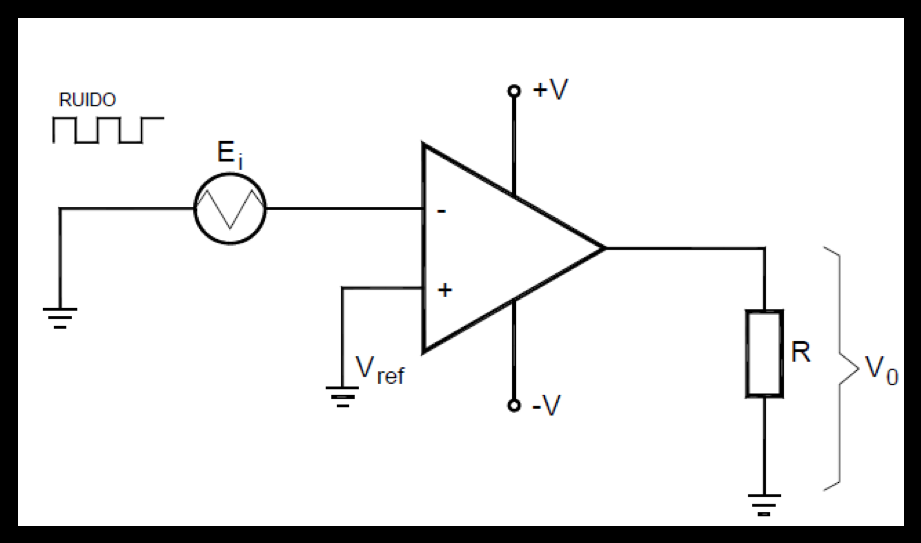
\includegraphics[width = 8cm, height = 5cm]{Inverting.png}
\centering \linebreak \linebreak Figure 1.0: Zero-crossing inverting level detector.
\end{figure} \hfill

\begin{figure}[H]
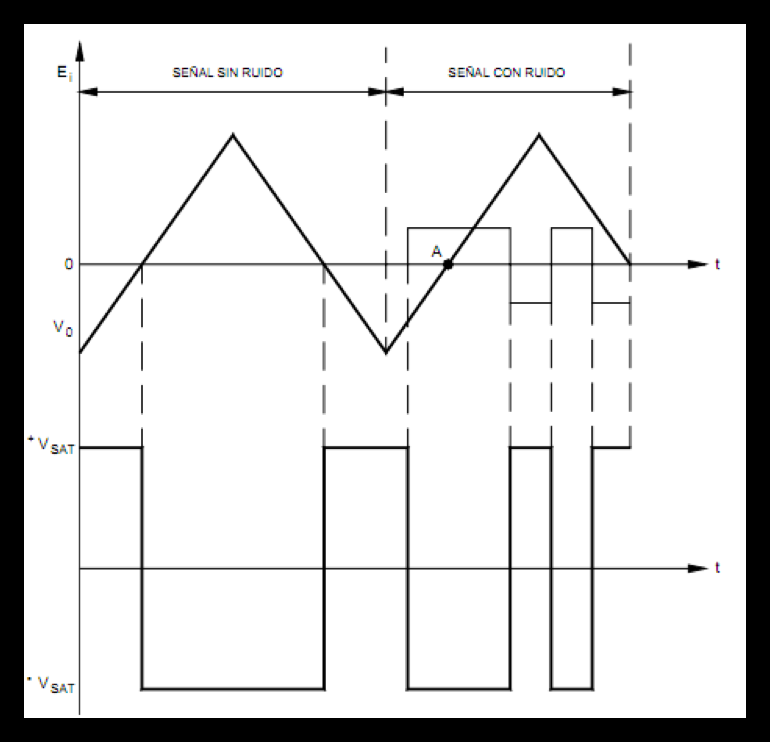
\includegraphics[width = 8cm, height = 5cm]{Inverting-graph.png}
\centering \linebreak \linebreak Figure 1.1: Input and output waveform of Figure 1.0.
\end{figure} \hfill
\end{multicols} 

\begin{multicols}{2}
\begin{figure}[H]
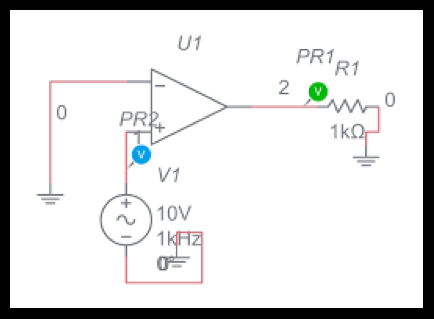
\includegraphics[width = 8cm, height = 5cm]{Non.png}
\centering \linebreak \linebreak Figure 1.2: Zero-crossing non-inverting level detector.
\end{figure} \hfill

\begin{figure}[H]
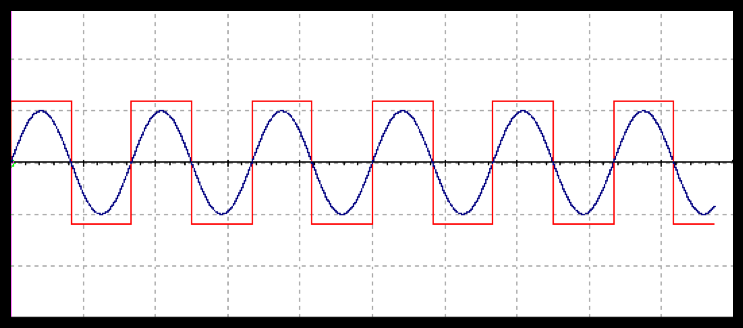
\includegraphics[width = 8cm, height = 5cm]{Non-graph.png}
\centering \linebreak \linebreak Figure 1.3: Input and output waveform of Figure 1.2.
\end{figure} \hfill
\end{multicols} 

\pagebreak

\subsection{Level Detector With Hysteresis:}

Also know as Schmidt Trigger, the circuit of the Figure 1.1.0 corresponds to a level detector with Hysteresis. The operational amplifier is powered between +Vcc and -Vcc. Note that the Operational amplifier does not receive negative feedback and instead has positive feedback through $R_{2}$. In the level detector with hysteresis, the output of the operational amplifier oscillates between the two possible saturation states, +Vcc and -Vcc, according to the values take by the input signal $V_{g}$ in relation to the reference voltage $V_{ref}$, and to the values ​​of the resistance network $R_{1}$ and $R_{2}$. \hfill \break

\begin{figure}[H]
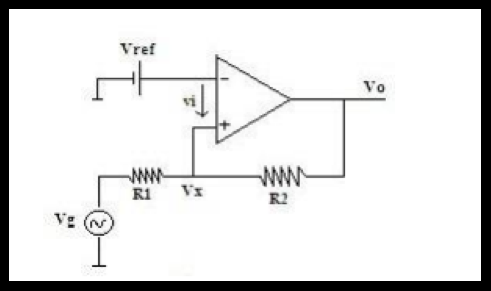
\includegraphics[width = 8cm, height = 5cm]{hysteresis.png}
\centering \linebreak \linebreak Figure 1.1.0: Level detector with hysteresis configuration.
\end{figure} \hfill

In an operational amplifier, when $V_{i}$ $>$ 0 is satisfied, the output $V_{o}$ saturates negatively ( $V_{o}$ = -$V_{sat}$ ); on the other hand if $V_{i}$ $<$ 0 then the output $V_{o}$ saturates positively ( $V_{o}$ = $V_{sat}$ ). According to the previous circuit, $V_{i}$ = $V_{x}$ - $V_{ref}$. To determine $V_{ix}$ we use the equivalent circuit shown below: \hfill \break

\begin{figure}[H]
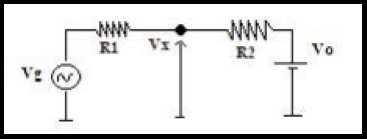
\includegraphics[width = 8cm, height = 5cm]{op1.png}
\centering \linebreak \linebreak Figure 1.1.1: Circuit equivalent for Figure 1.1.0.
\end{figure} \hfill

Applying the superposition theorem results:

\begin{ceqn}
\begin{align*}
V_{x}\ =\ (\ V_{g}\ \cdot\ \frac{R_{2}}{R_{1}\ +\ R_{2}}\ )\ +\ (\ V_{o}\ \cdot\ \frac{R_{1}}{R_{1}\ +\ R_{2}}\ )
\end{align*}
\end{ceqn} \hfill

\pagebreak

To analyze the level detector we assume an initial state in negative saturation ( $V_{o}$ = -Vcc ) and that $V_{g}$ is a variable signal that is increasing from negative values, so that $V_{x}$ $<$ $V_{ref}$ is fulfilled. Figure 1.1.2 shows the relationship between $V_{o}$ and $V_{g}$: \hfill \break

\begin{figure}[H]
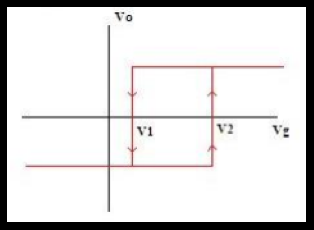
\includegraphics[width = 8cm, height = 5cm]{transfer.png}
\centering \linebreak \linebreak Figure 1.1.2: Transfer function for the hysteresis circuit.
\end{figure} \hfill

\subsection{Practical Application:}

The most common use of a zero crossing detector is to govern the application of alternating current to a load, for example to reduce the intensity of a bulb (dimmer): the alternating current is a sine wave that is circulating in one direction and in another at a rate of 60 cycles per second, then each half period passes through zero, that is, its intensity is zero. In AC circuits to decrease the power of the load, the zero crossing is detected, a pause is taken and a TRIAC is triggered; During the pause, the load remains off, when the TRIAC is triggered, the load is turned on and stays on until the vol-point goes through zero, automatically turning off the TRIAC. The period of the alternating cycle at 60 cycles / second is 16.67 milliseconds, every 8.3 milliseconds crosses zero; if a circuit detects zero crossing and pauses 4.15 milliseconds then the load is halved.

\pagebreak
